% !TEX program = lualatex -synctex=1 --interaction=nonstopmode -file-line-error -shell-escape
% !TEX encoding = UTF-8
% !BIB program = bibtex
% !TEX spellcheck = en_US
\documentclass[12pt,twoside]{article}

\usepackage{nicefrac}
\usepackage{./mystyle}

\graphicspath{{images/}{plots/}}

\newcommand{\institution}{Universitas Columbiae}
\newtheorem{theorem}{Argument}

\title{PHYS6080 Scientific Computing}
\author{Qi Zhang}
\date{\today}

\makeatletter
\let\thetitle\@title
\let\theauthor\@author
\let\thedate\@date
\makeatother

\begin{document}

% See https://www.overleaf.com/latex/templates/operating-systems-laboratory/wswyyqztyryp
\begin{titlepage}
    \centering
    \vspace*{2 cm}
    
\includegraphics[height=5cm]{logo}\\[1.0 cm]
    \textsc{\LARGE \institution}\\[2.0 cm]
    \textsc{\Large Autumn 2022}\\[0.5 cm]
    \rule{\linewidth}{0.2 mm}\\[0.4 cm]
    {\huge \bfseries \thetitle}\\
    \rule{\linewidth}{0.2 mm}\\[1.5 cm]

    \begin{minipage}{0.4\textwidth}
        \begin{flushleft} \large
            \emph{Submitted To:}\\
            Robert Mawhinney\\
            \href{mailto:rdm10@columbia.edu}{rdm10@columbia.edu}\\
            Professor\\
            Physics Department\\
        \end{flushleft}
    \end{minipage}~
    \begin{minipage}{0.4\textwidth}
        \begin{flushright} \large
            \emph{Submitted By:} \\
            \theauthor\\
            \href{mailto:qz2280@columbia.edu}{qz2280@columbia.edu}\\
            APAM Department\\
            \thedate\\
        \end{flushright}
    \end{minipage}\\[2 cm]
\end{titlepage}

\newpage


\section{Use the velocity Verlet algorithm to study liquid argon}

For this problem set, you should implement the velocity Verlet algorithm and use
it to study liquid argon. You should use the
velocity Verlet algorithm for your simulations. It is self-starting, making it slightly
easier to use than the simple Verlet algorithm in Verlet's original paper.

This is a study of a collection of classical particles interacting through a Lennard--Jones
potential, a central force potential. The evolution of this system according to Newton's
Laws represent a microcanonical ensemble, since the energy is fixed. The temperature of the
system can be found from the average kinetic energy.

In writing your program, there are a number of issues to consider:

\begin{enumerate}
    \item The system should be put in a box of size $L$ on a side. The desired density and
          input number of particles will determine the box size. Periodic boundary
          conditions should be used.
    \item The energy and force for particle $a$ due to particle $b$ should be calculated
          using the ``nearest image'' of particle $b$.
    \item While integrating the equations of motion, some particles will move out of the
          box. By a shift of $L$ in the appropriate coordinate, the particle can be brought
          back into the box.
    \item The initial state of the system must be chosen. You can easily choose the
          velocities $\vec{v}$ so that each component is uniformly distributed between
          $-v_\text{max}$ and $v_\text{max}$. After choosing the velocities for each
          particle, shift all velocities so that the velocity of the center of mass is zero.
          Alternatively, you can place all the particles initially at rest, and then they
          will acquire velocities as the system thermalizes.

          Putting the particles at random positions inside the box will generally result in
          very large potential energies. A few relaxation steps, moving each particle
          individually a small distance in the direction of the force acting on it, will
          dramatically decrease the potential energy. You can also arrange the particles in
          a somewhat regular pattern to avoid any two particles being too close together.
          The important point is that the initial configuration does not matter, provided
          there are no particles close enough to each other that the $\frac{ 1 }{ r^{12} }$
          term in the potential becomes large.
    \item Once chosen, the total energy will remain fixed, provided your algorithm is
          working correctly. The temperature will be set, after thermalization, by the
          resulting balance between kinetic and potential energy.
\end{enumerate}

You should check your program by studying whether it conserves energy and whether the
particles motion is reversible, i.e., whether the system returns to an earlier state when
the velocities are reversed, and the molecular dynamics restarted.

Once you believe your program is working, you should reproduce the values for pressure and
internal energy found by Verlet for $\rho = 0.75$ and $T = 1.069$. You can fine-tune the
temperature by small rescaling of the velocities or by moving particles a small amount in
the direction of the force they are experiencing, i.e., moving them downhill. (Remember that
you need to run the molecular dynamics for some time after such an adjustment to let the
system come back into thermal equilibrium.)

To get reasonable accuracy for $T$ and $P$, runs of a few thousand molecular dynamics steps
should be sufficient after thermalization. You do not need to reproduce the temperature to
precisely $1.069$.

Some additional features you should have in your program and results you should produce are:

\begin{enumerate}
    \item You should be able to write the position and velocity of all the particles to a
          file, at intervals of your choosing. You should also be able to read this file in
          and continue your simulation. This will allow you to add more molecular dynamics
          time to a simulation, without re-starting from an unthermalized state.
    \item Record in a file the measurements necessary to determine the pressure, via the
          virial theorem, every $10$ molecular dynamics steps. We will use these later to
          determine the statistical errors on your measurements.
    \item Determine the velocity distribution of the particles by recording them after every
          $10$ molecular dynamics steps. Does it agree with the expected Maxwell distribution?
\end{enumerate}

\subsection{Applying periodic boundary conditions}\label{ssec:pbcs}

Suppose we have a system of \(N\) particles with number density \(\rho\), thus the
box size will be

\begin{equation}\label{eq:L}
    L = \biggl( \frac{ N }{ \rho } \biggr)^{1 / 3}.
\end{equation}

If we want to impose the periodic boundary conditions (PBCs) here, we should adopt the
nearest image convention (NIC) or minimum image convention (MIC). What is an image? First,
we should emphasize that we could not do simulations in an infinitely large box (cell) in
molecular dynamics (MD)
simulations. The most common solution is to take one cell (we will call it ``center cell''
in the following text) to simulate and imagine an infinitive number of image cells
surrounding it, where each image cell is a replica of the center cell. The image cells can
reduce or eliminate boundary effects by providing every particle an equivalent surrounding
environment of particles as if it were in the bulk, no matter where they are in the center
cell.

\begin{figure}[h]
    \centering
    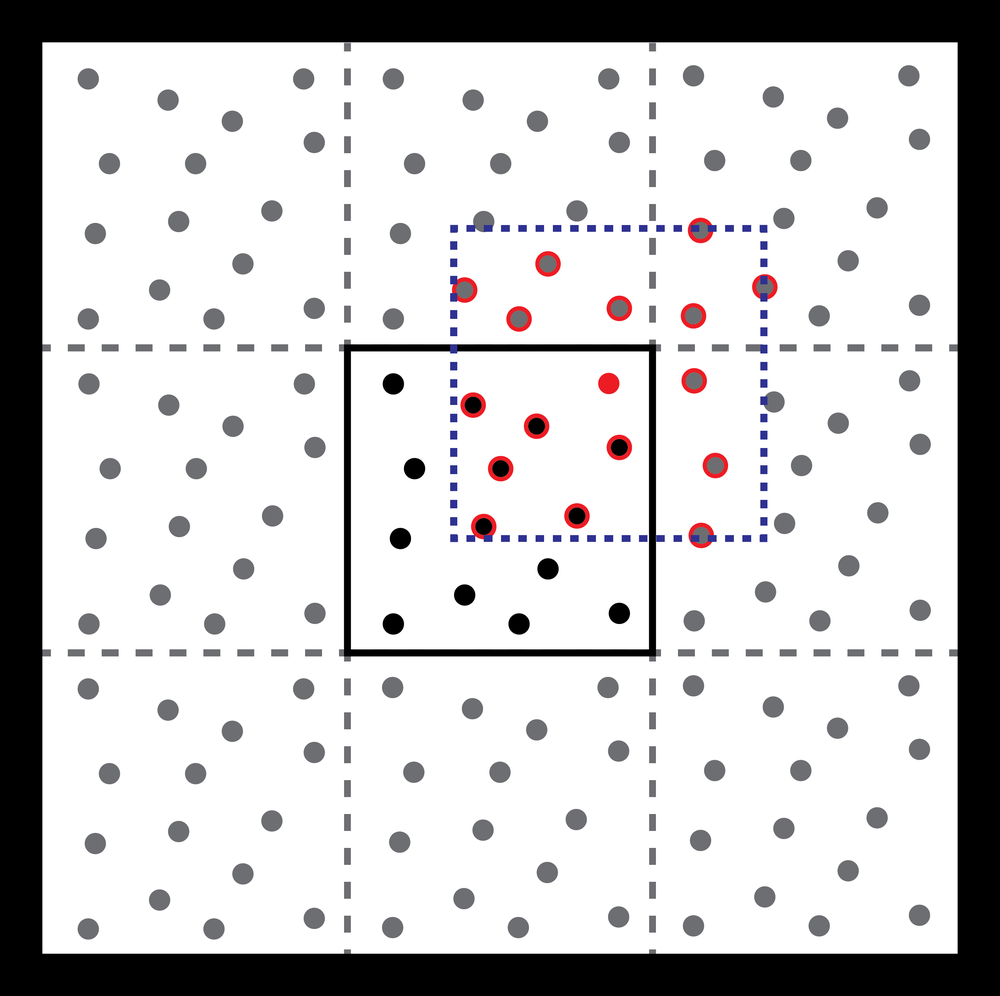
\includegraphics[width=0.5\textwidth]{nic}
    \caption{A center cell surrounded by \(8\) more image cells with the same
        particles' relative locations and movements. Figure is from \cite{matlab}.}
    \label{fig:nic}
\end{figure}

When applying PBCs, particles near the edge of the cells often interact
with an image particle rather than a particle in the cell. For example, we can create the
situation shown below.
In Figure~\ref{fig:nic}, the black border box is our center cell, and the \(8\) others are
its replica. The relative positions and velocities of the particles in these image cells
are exactly the same as their originals in the center cell. The red particle in the
upper left corner of the center cell only interacts with its neighbors: some of the
particles in the center cell plus some of the image particles in the image cells.
We call the box enclosing the red particle's neighbors a ``virtual image cell''.
The size of the virtual image cell (cutoff radius) is usually chosen as \(L / 2\)
of the center cell. That is, any particle which is more than \(L / 2\) away from the
red particle in any direction is not included in the virtual image cell.
If the cutoff radius is larger than \(L / 2\), it may lead to
unphysical self-interactions, sometimes called an artifact.

Another aspect of the PBCs is that when a particle hits a cell wall, instead of bouncing
back, it reappears on the other side of the cell (the topology of a torus), or we can
treat it as an image particle from an adjacent cell enters the current cell.
So the number of particles in a cell never increases or decreases in this case.

\begin{algorithm}
    \caption{Find the nearest image of particle \(b\) which can interact with particle \(a\).}
    \label{lst:nic}
    \begin{juliacode}
        Δ𝐫 = b.coordinates - a.coordinates
        coordinates = map(b.coordinates, Δ𝐫) do rᵢ, Δrᵢ
            if Δrᵢ > L / 2
                rᵢ - L
            elseif Δrᵢ < -L / 2
                rᵢ + L
            else  # |Δrᵢ| <= L / 2
                rᵢ  # Do not shift
            end
        end
    \end{juliacode}
\end{algorithm}

So how do we express the PBCs in mathematical and programming languages?
Suppose we have two particles, \(a\) and \(b\), both in the center cell,
and \(a\) is the particle in which we
are interested. The vector pointing from \(a\) to \(b\) is the difference between
their positions:
%
\begin{equation}
    \bm{r} = \bm{r}_b - \bm{r}_a.
\end{equation}
%
For any component \(r_\alpha\) of \(\bm{r}\), where \(\alpha = 1, 2, 3\), if its absolute value
is larger than \(L / 2\), then we know \(b\) is too far from \(a\) to have effects on it,
so we should shift \(b\) closer to \(a\) in the corresponding dimension:
%
\begin{equation}
    \begin{cases}
        r_{b, \alpha} - L, & \text{if } r_\alpha > L / 2,                  \\
        r_{b, \alpha} + L, & \text{if } r_\alpha < -L / 2,                 \\
        r_{b, \alpha},     & \text{if } \lvert r_\alpha \rvert \leq L / 2,
    \end{cases}
\end{equation}
%
where \(r_{b, \alpha}\) is the component of the position of particle \(b\) in the
corresponding dimension.
The Julia code for the above procedure looks like Snippet~\ref{lst:nic}.
The code will return a \code{Vector} representing the new position of particle \(b\).

If \(b\) is not in the same cell as \(a\), we need first shift \(b\) back to the cell where
\(a\) locates. That is,
%
\begin{equation}\label{eq:pbcs}
    (r_{b, \alpha} + 2L) \mod L,
\end{equation}
%
where adding \(2L\) is to catch any runaway particles\cite{Adrian} with \(r_{b, \alpha} < -L\).
The code representing \eqref{eq:pbcs} is in Snippet~\ref{lst:pbcs}.
%
\begin{algorithm}
    \caption{Move particle \(b\) back to the center cell.}
    \label{lst:pbcs}
    \begin{juliacode}
        f(rᵢ) = mod(rᵢ, L)
        b.coordinates = map(f, b.coordinates)
    \end{juliacode}
\end{algorithm}
%
Here Julia already provides the modulo function (it works for floating point numbers)
\href{https://docs.julialang.org/en/v1/base/math/#Base.mod}{\code{mod}}. Python and C++
also have similar functions. And since \(L\) is always positive, we do not need to worry
about some nasty cases.
In the snippet, we \code{map} function \code{f} over
each component of the \(b\)'s position.

\begin{figure} % 2 subfigures
    \centering
    \begin{minipage}[t]{0.5\linewidth}
        \centering
        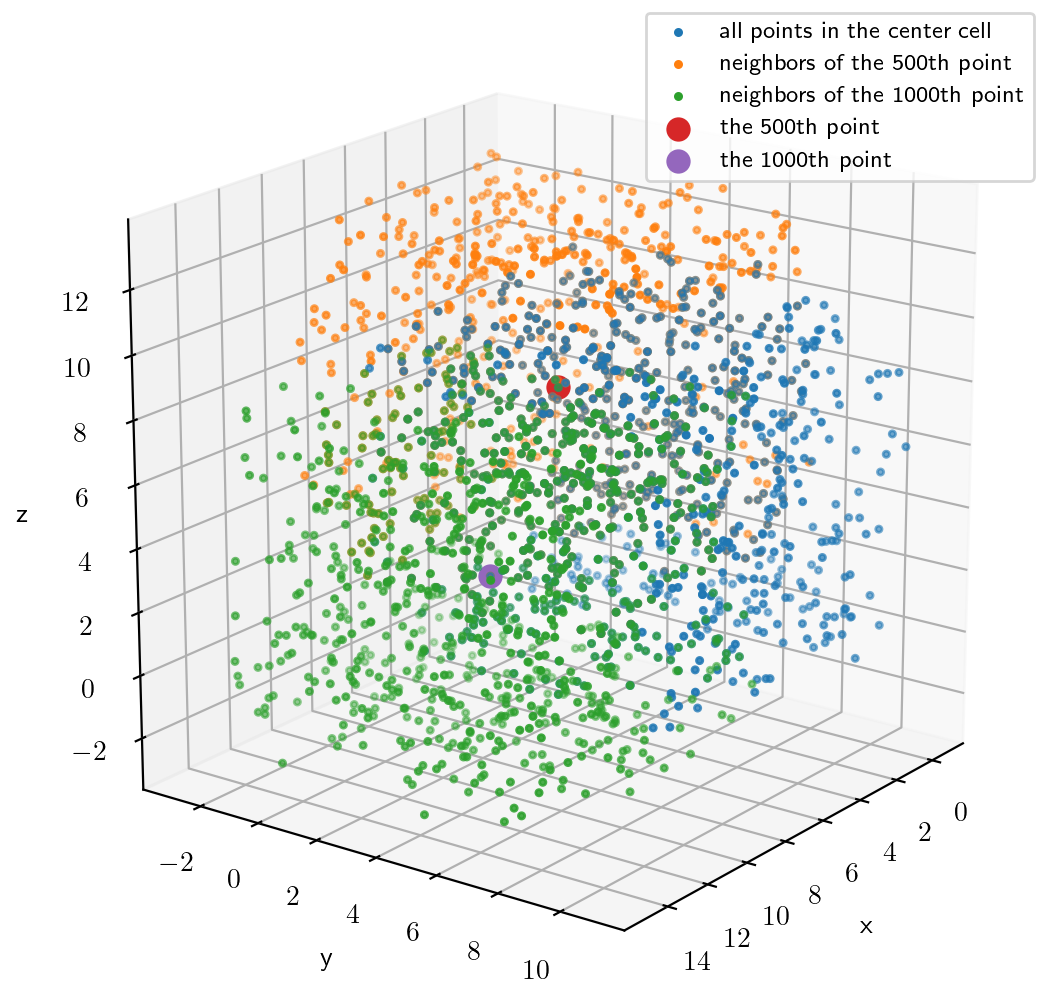
\includegraphics[width=\linewidth]{neighbors_profile}
        \subcaption{Viewing from one angle of neighbors of the selected particles.}
        \label{fig:neighbors:a}
    \end{minipage}
    \hfill
    \begin{minipage}[t]{0.5\linewidth}
        \centering
        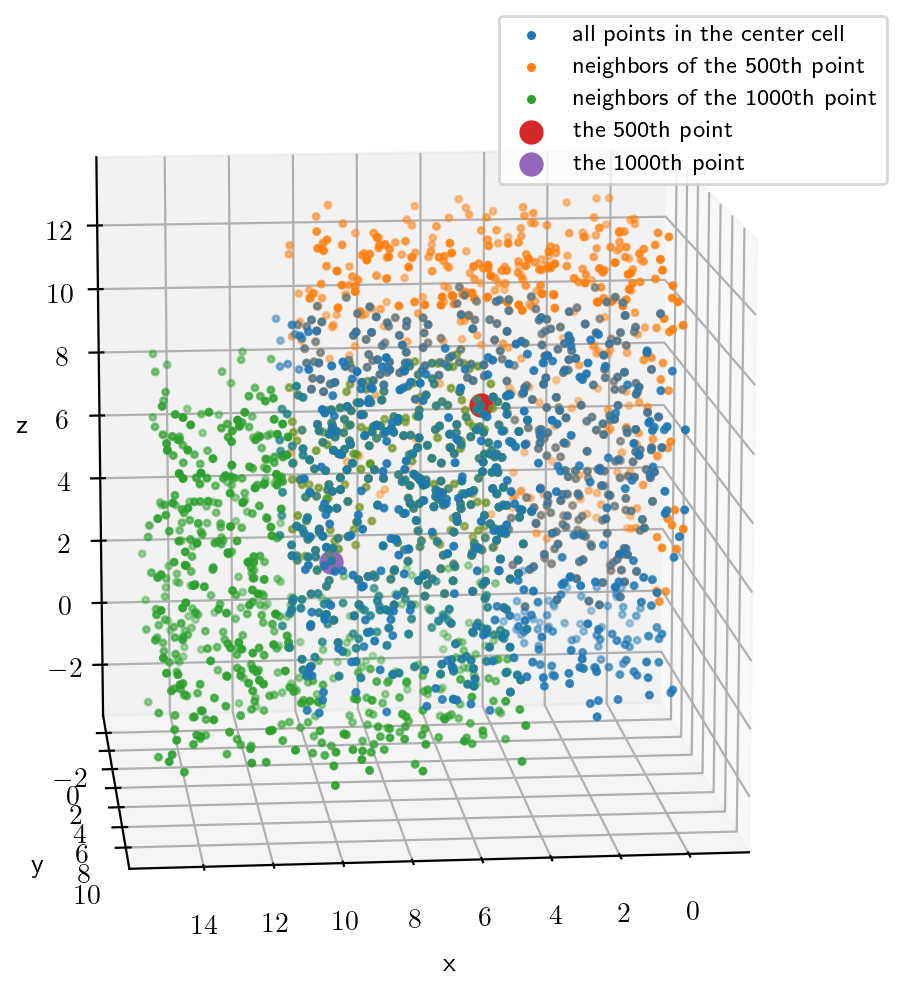
\includegraphics[width=\linewidth]{neighbors_front}
        \subcaption{Viewing from another angle of neighbors of the selected particles.}
        \label{fig:neighbors:b}
    \end{minipage}
    \caption{A system of \(1000\) particles with \(L \approx 11\). The blue points denote all
        the points in the center (original) cell, and the red and purple spheres are the
        \(500\)th and \(1000\)th particle among them. The orange and green points are the
        neighbors of these points which have interactions with them.}
    \label{fig:neighbors}
\end{figure}

To ensure that we have the correct neighbors, we need to plot the positions of these particles.
As shown in Figure \ref{fig:neighbors}, we have a system of \(1000\) particles with
\(\rho = 0.75\), so \(L \approx 11\). The blue points denote all
the points in the center (original) cell, and the red and purple spheres are the
\(500\)th and \(1000\)th particles among them. The orange and green points are the
neighbors of these points which have interactions with them. That is, they are bounded by a
cubic whose centers are the \(500\)th and \(1000\)th particles,
with size \(L \approx 11\) in each dimension.
There are \(999\) points in both orange and green ``clouds'', and they do have overlaps
with the blue ``cloud''. From this, we know there is no double counting in our algorithm.

The syntax in Snippet \ref{lst:nic} and \ref{lst:pbcs} may confuse users as we
have not mentioned how we represent particles in
code. In our code, a \code{Particle} is simply a \code{mutable struct} wrapping two
\code{MVector}s (position and velocity), each with three \code{Float64} values, as shown in
Snippet~\ref{lst:particle}. So \code{b.position} (\code{b.velocity}) is how we access the
stored data of its position (velocity).

\begin{algorithm}
    \caption{The definition of a particle in our code.}
    \label{lst:particle}
    \begin{juliacode}
        using StaticArrays: MVector

        mutable struct Particle
            coordinates::MVector{3,Float64}
            velocity::MVector{3,Float64}
        end
    \end{juliacode}
\end{algorithm}

\subsection{Force calculation}

Now let us talk about the Lennard--Jones potential.
The original form of the two-particle potential would look like~\eqref{eq:uljunit}:
%
\begin{equation}\label{eq:uljunit}
    u(r_{ij}) = 4 \varepsilon \biggl( \Bigl( \frac{ \sigma }{ r_{ij} } \Bigr)^{12}
    -\Bigl( \frac{ \sigma }{ r_{ij} } \Bigr)^6 \biggr),
\end{equation}
%
where the parameters for \ce{Ar} are $\varepsilon = \SI{0.0104}{\electronvolt}$,
$\sigma = \SI{3.40}{\angstrom}$, and $m = \SI{39.948}{\atomicmassunit}$, where
$\si{\atomicmassunit}$ is the atomic mass unit.
In the dimensionless form,
\eqref{eq:uljunit} would look like~\eqref{eq:ulj} and the force would
look like~\eqref{eq:flj}.
%
\begin{align}
    u(r_{ij})                      & = 4 \biggl( \Bigl( \frac{ 1 }{ r_{ij} } \Bigr)^{12}
    -\Bigl( \frac{ 1 }{ r_{ij} } \Bigr)^6 \biggr), \label{eq:ulj}                        \\
    \frac{ d^2 \bm{r}_i }{ d t^2 } & = 48\sum_{j \neq i} (\bm{r}_i - \bm{r}_j)
    \biggl( \Bigl( \frac{ 1 }{ r_{ij} } \Bigr)^{14}
    -\frac{ 1 }{ 2 } \Bigl( \frac{ 1 }{ r_{ij} } \Bigr)^8 \biggr). \label{eq:flj}
\end{align}
%
And the numerical gradient of~\eqref{eq:ulj} is
%
\begin{equation}\label{eq:dudr}
    \begin{bmatrix}
        \nicefrac{ \partial u }{ \partial x } \\
        \nicefrac{ \partial u }{ \partial y } \\
        \nicefrac{ \partial u }{ \partial z }
    \end{bmatrix}
    \Rightarrow
    \begin{bmatrix}
        \nicefrac{ \bigl( u(\bm{r} + dx \hat{\bm{x}}) - u(\bm{r}) \bigr) }{ dx } \\
        \nicefrac{ \bigl( u(\bm{r} + dy \hat{\bm{y}}) - u(\bm{r}) \bigr) }{ dy } \\
        \nicefrac{ \bigl( u(\bm{r} + dz \hat{\bm{z}}) - u(\bm{r}) \bigr) }{ dz }
    \end{bmatrix}.
\end{equation}
%
I found in the notes, equation \eqref{eq:flj} is off by a factor of $48$.
Only after adding it could make \eqref{eq:dudr} and \eqref{eq:flj} match.
I suppose that this is because we basically treat
$\varepsilon$, $\sigma$, and $m$ (the mass of each particle) as $1$ here (though they
are not). So in Snippet~\ref{lst:gradient} I define the $\nabla u$ and the acceleration
particle $a$ experiences (induced only by particle $b$) as below.
%
\begin{algorithm}
    \caption{The gradient of the Lennard--Jones potential and the acceleration
        $d^2 \bm{r}_a / d t^2$. Note the factor $48$ and the negative sign.}
    \label{lst:gradient}
    \begin{juliacode}
        function potential_gradient(𝐫ᵢⱼ)
            rᵢⱼ = norm(𝐫ᵢⱼ)
            return 48𝐫ᵢⱼ * (inv(rᵢⱼ^8) / 2 - inv(rᵢⱼ^14))
        end

        function Acceleration(a::Particle)
            return function (b::Particle)
                return Acceleration(-potential_gradient(a.position - b.position))
            end
        end
    \end{juliacode}
\end{algorithm}
%
The corresponding unit test is shown in Snippet~\ref{lst:ut_gradient}.
%
\begin{algorithm}
    \caption{The unit test of function \code{potential_gradient}.}
    \label{lst:ut_gradient}
    \begin{juliacode}
        𝐫 = [4, 5, 6]  # Distance between two particles
        δ = 0.00005
        u₀ = potential_energy(𝐫)  # Potential energy between the two particles
        for i in 1:3  # Loop over each component of vector `𝐫`
            Δ𝐫 = zeros(3)
            Δ𝐫[i] = δ  # Set the `i`th component of `Δ𝐫` to be `δ`
            u₁ = potential_energy(𝐫 + Δ𝐫)  # New potential energy between the two particles
            @test (u₁ - u₀) / δ - potential_gradient(𝐫)[i] < 1e-8
        end
    \end{juliacode}
\end{algorithm}
%
The negative sign indicates the force is the negative gradient of the potential.
To get the total potential energy of the swarm of particles, we sum up all the $i$'s
and $j$'s (except for $j = i$) in~\eqref{eq:U}:
%
\begin{equation}\label{eq:U}
    U = \frac{ 1 }{ 2 }\sum_{\substack{i, j\\ j \neq i}} u(r_{ij}).
\end{equation}
%
Note the $\frac{ 1 }{ 2 }$ factor in \eqref{eq:U} since we count $i$ and $j$ twice.
Snippet \ref{lst:U} does the same thing:

\begin{algorithm}
    \caption{Calculate the total Lennard--Jones potential energy of a swarm of particles.}
    \label{lst:U}
    \begin{juliacode}
        function potential_energy(particles::Vector{Particle})
            return 1 / 2 * sum(eachindex(particles)) do i
                sum(filter(!=(i), eachindex(particles))) do j
                    potential_energy(particles[i], particles[j])
                end
            end
        end
    \end{juliacode}
\end{algorithm}

Similarly, we need to calculate the total force (acceleration) of all the other particles
enforced on one particle, as shown in \eqref{eq:flj}. Now we need to employ the
\code{list_neighbors} function we used to calculate one particle's neighbors and plotted
Figure \ref{fig:neighbors}, as shown in \ref{lst:flj}.
%
\begin{algorithm}
    \caption{Calculate the total Lennard--Jones force a particle experiences.}
    \label{lst:flj}
    \begin{juliacode}
        function acceleration(cell::Cell, particle::Particle)
            neighbors = list_neighbors(cell, particle)
            return sum(Acceleration(particle), neighbors)
        end
    \end{juliacode}
\end{algorithm}
%

\subsection{Integrators}

There exist many algorithms for integrating ordinary differential equations.
In this section, we consider the particular case of numerically integrating the equations of
motion for a dynamical system described by a time-independent Hamiltonian, i.e., the
classical many-particle system as a microcanonical ensemble.
Here, we use the velocity Verlet algorithm as our integrator.
The mathematical expression of the algorithm is shown in \eqref{eq:vvr} and \eqref{eq:vvv}.
%
\begin{align}
    \bm{r}(t + \Delta t) & = \bm{r}(t) + \bm{v}(t) \Delta t + \frac{ \bm{a}(t) }{ 2 } \Delta t^2,\label{eq:vvr} \\
    \bm{v}(t + \Delta t) & = \bm{v}(t) + \frac{ \bm{a}(t) + \bm{a}(t + \Delta t) }{ 2 } \Delta t,\label{eq:vvv}
\end{align}
%
where $\Delta t$ is the length of each time step, $\bm{r}(t + \Delta t)$,
$\bm{v}(t + \Delta t)$, and $\bm{a}(t + \Delta t)$
are the coordinates, velocity, and acceleration of the particle at time $t + \Delta t$.
In our dimensionless system, the acceleration and the force have the same value,
where the method of calculating forces is described in section \ref{ssec:force}.
The force at time $t$ is calculated by all the positions of the particles at time $t$.

The standard implementation scheme of the velocity Verlet algorithm is:
%
\begin{enumerate}
    \item Calculate $\bm{v}(t + \nicefrac{\Delta t}{2}) = \bm{v}(t) + \frac{1}{2} \bm{a}(t) \Delta t$;
    \item Calculate $\bm{r}(t + \Delta t) = \bm{r}(t) + \bm{v}(t + \nicefrac{\Delta t}{2}) \Delta t$;
    \item Derive $\bm{a}(t + \Delta t)$ from the Lennard--Jones potential using $\bm{r}(t + \Delta t)$;
    \item Calculate $\bm{v}(t + \Delta t) = \bm{v}(t + \nicefrac{\Delta t}{2}) + \frac{1}{2} \bm{a}(t + \Delta t) \Delta t$.
\end{enumerate}
%
The corresponding code for the above algorithm is shown in Snippet~\ref{lst:take_one_step},
defined by function \code{take_one_step!}.
%
\begin{algorithm}
    \caption{Move all particles one step forward in the simulation cell with time step
        $\Delta t$, using the velocity Verlet integrator.}
    \label{lst:take_one_step}
    \begin{juliacode}
        function take_one_step!(particles, box::Box, Δt, ::VelocityVerlet)
            for (particle, 𝐟) in zip(particles, force(particles, box))
                particle.velocity += 𝐟 * Δt / 2  # 𝐯(t + Δt / 2)
                particle.coordinates += particle.velocity * Δt  # 𝐫(t + Δt)
                map!(Base.Fix2(mod, box.side_length), particle.coordinates, particle.coordinates)  # Move `𝐫` back to `0 - L` range
            end
            for particle in particles
                𝐟 = force(particle, particles, box)  # 𝐚(t + Δt)
                particle.velocity += 𝐟 * Δt / 2  # 𝐯(t + Δt)
            end
            return particles
        end
    \end{juliacode}
\end{algorithm}
%
The input \code{particles} and \code{box} are the simulation particles and the cell we
are interested in, with its number density to be $0.75$ here. And each time step
$\Delta t$ is $0.032$ (which Verlet used in his simulation). For \ce{Ar}, it corresponds
to the real world time of
%
\begin{equation}
    t_\textnormal{real} = t \sqrt{\frac{ m \sigma^2 }{ 48 \varepsilon }}
    \approx 0.032 \times \num{3.112e-13}
    \approx \qty{9.96e-15}{\second},
\end{equation}
%
which is roughly \qty{1e-14}{\second}, as claimed by Verlet\cite{Verlet}.
We should notice that the time step cannot be too large, which will result in force
increasing rapidly, and within each time step, the particles can come too close,
causing our simulation hard to converge.

\subsection{Loggers}

To track the positions and velocities of all the particles, we need some loggers.
Here we define two types, a \code{Step} type which represents each step of the molecular
dynamics, and a \code{Logger} type which stores all the \code{Step}s we have run,
as shown in Snippet~\ref{lst:logger}.

\begin{algorithm}
    \caption{The \code{Step} and \code{Logger} types that track each step of the
        molecular dynamics.}
    \label{lst:logger}
    \begin{juliacode}
        struct Step{N}
            Δt::Float64
            snapshot::SVector{N,Particle}
        end

        struct Logger{N}
            history::ElasticVector{Step{N}}
        end
    \end{juliacode}
\end{algorithm}

To track and continue our simulation, we also need to add two new methods to function
\code{take_n_steps!}, as shown in Snippet~\ref{lst:trackncontinue}.
In the first method, all steps are saved in variable \code{logger} if we start a new
molecular dynamics simulation, and the second method indicates we are restarting an
existing simulation with all previous steps from the variable \code{logger}.

\begin{algorithm}
    \caption{To save and restart MD simulations we need to track these steps
        in the variable \code{logger}.}
    \label{lst:trackncontinue}
    \begin{juliacode}
        function take_n_steps!(
            logger::Logger{N}, particles, box::Box, n, Δt, ::VelocityVerlet
        ) where {N}
            @showprogress for _ in 1:n
                take_one_step!(particles, box, Δt, VelocityVerlet())
                push!(logger.history, Step(Δt, SVector{N}(deepcopy(particles))))
            end
            return particles
        end
        function take_n_steps!(logger::Logger, box::Box, n, Δt, ::VelocityVerlet)
            particles = logger.history[end].snapshot
            return take_n_steps!(logger, particles, box, n, Δt, VelocityVerlet())
        end
    \end{juliacode}
\end{algorithm}

We may use Julia's serialization library \code{Serialization} to
serialize (save) and deserialize (load) the logger. Or, we can use third-party packages
such as \href{https://github.com/JuliaIO/JLD.jl}{\code{JLD.jl}} and
\href{https://github.com/JuliaIO/JLD2.jl}{\code{JLD2.jl}}.
But these file formats are binary, so they are not human readable.
If we want to read these files by ourselves, serializing them into readable formats
is also necessary. Here, we adopt the JSON format, which
is an open standard and data interchange format that uses human-readable text to
store and transmit data objects. With the help of it, we can store the locations
and velocities of the particles into a JSON file. The corresponding code is shown in
Snippet~\ref{lst:json}.

\begin{algorithm}[H]
    \caption{Code to save (load) the information to (from) a JSON file.}
    \label{lst:json}
    \begin{juliacode}
        function Base.Dict(particle::Particle)
            return Dict("coordinates" => particle.coordinates, "velocity" => particle.velocity)
        end

        Base.print(io::IO, particle::Particle) = JSON.print(io, Dict(particle))
        function Base.print(io::IO, particles::AbstractVector{Particle})
            JSON.print(io, map(Dict, particles))
        end

        function save(filename, data)
            open(filename, "w") do io
                print(io, data)
            end
        end

        function load(filename)
            return open(filename, "r") do io
                JSON.parse(io)
            end
        end
    \end{juliacode}
\end{algorithm}

\subsection{Velocity-rescaling thermostat}

Now let us perform the molecular dynamics simulation.
First, we need to define our system. We select a system of $1000$ particles,
with number density $\rho = 0.75$, as in Vertlet\cite{Verlet}'s paper.
According to~\eqref{eq:L}, the box's side length will be about $11.006 \sigma$.
We also need to set the initial positions and velocities of the particles.
We choose all the particles spaced by a constant distance, larger than $1$
to avoid the initial potential energy being too large (see~\eqref{eq:uljunit}),
in each direction, and all velocities to be zero.
We will first run $5000$ MD steps to see the trend of the potential energy
and kinetic energy.
The corresponding code is in Snippet~\ref{lst:md5000}.
%
\begin{algorithm}
    \caption{Running $5000$ MD steps.}
    \label{lst:md5000}
    \begin{juliacode}
        particles = [Particle(rand(3), rand(3)) for _ in 1:1000]  # Generate 1000 particles
        box = CubicBox(length(particles), 0.75)  # Put them in a cubic box to s.t. number density = 0.75
        init!(particles, box, Even(), Uniform(zeros(Velocity)))  # Set the initial positions and velocities
        logger = Logger(length(particles))  # Start a logger tracking the MD steps
        Δt = 0.032  # The length of each time step
        take_n_steps!(logger, particles, box, 5000, Δt, VelocityVerlet())  # Run MD simulation
    \end{juliacode}
\end{algorithm}
%
After the code finishes, we plot the dimensionless kinetic energy, potential energy,
and total energy as a function of simulation time $t$ in Figure~\ref{fig:md5000}.
After $5000$ steps, which is around $160$ units of dimensionless time and
\qty{5e-11}{\second} in real world time, we seem to already reach thermal equilibrium.
As the figure shows, after $t = 40$ we can see a substatial decrease in the potential energy
and increase in the kinetic energy, while the total energy keeps almost the same for
the whole time, as it should be.
%
\begin{figure}
    \centering
    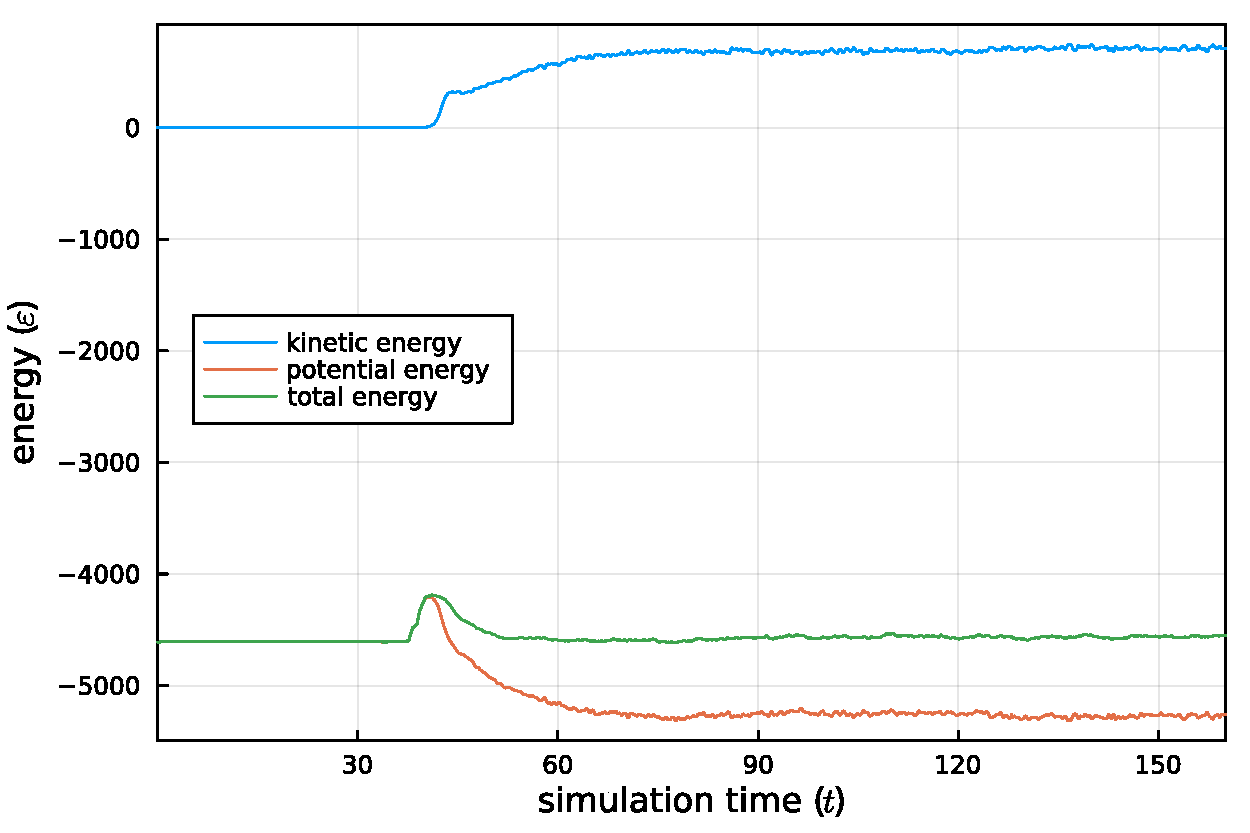
\includegraphics[width=0.8\textwidth]{e-t-no-thermostat}
    \caption{The dimensionless kinetic energy, potential energy, and total energy
        as a function of simulation time $t$.}
    \label{fig:md5000}
\end{figure}
%
To make sure the kinetic energy calculated using~\eqref{eq:kinetic} is correct, we compare
the difference between the last and the first steps of both the kinetic and potential
energies, $T_\text{last} - T_\text{initial} \approx 707.97$ and
$U_\text{last} - U_\text{initial} \approx -650.61$, so they are at the same magnitude,
the difference could come from the steady energy drifts caused by accumulation of
numerical errors.

The temperature is represented by Equation~\eqref{eq:T}
%
\begin{equation}\label{eq:T}
    T = \frac{ 16 }{ N } \sum_{i=1}^{N} \lvert \bm{v}_i \rvert^2,
\end{equation}
%
where $N$ is the number of particles, and $\bm{v}_i$ is the velocity of the $i$-th particle.
However, at $t = 160$, the temperature is only around $0.472$, far away from our desired
value: $1.069$. So we need to add more kinetic energy to our system. How do we do that?
We should use what is called a \emph{thermostat}, which is
a modification of the basic molecular dynamics scheme with the purpose of maintaining the
temperature constant (on average).

The simplest thermostat is a velocity-rescaling thermostat, as we can see, the equilibrium
temperature of our MD simulation after $5000$ steps are not equal to our desired value.
So we can multiply the velocities of the particles by a factor $\lambda$ to match our
desired temperature.
From Equation~\ref{eq:T}, we know that
%
\begin{equation}
    \lambda = \sqrt{\frac{ T_0 }{ T(t) }},
\end{equation}
%
where $T_0$ is the desired temperature and $T(t)$ is the current temperature as
calculated from the kinetic energy.
In this example, to match $T_0 = 1.069$, $\lambda = 1.505$.
And in Snippet~\ref{lst:thermostat}, we show the definition of our thermostat type
\code{VelocityRescaling} and rescaling function \code{apply_coupling!}.
%
\begin{algorithm}
    \caption{Definition of the velocity-rescaling thermostat and its application
        on the velocities of the particles.}
    \label{lst:thermostat}
    \begin{juliacode}
        abstract type Thermostat end
        struct VelocityRescaling <: Thermostat
            desired_temperature::Float64
        end

        function apply_coupling!(particles, thermostat::VelocityRescaling)
            t = temperature(particles)
            for particle in particles
                particle.velocity *= sqrt(thermostat.desired_temperature / t)
            end
            return particles
        end
    \end{juliacode}
\end{algorithm}

One problem with this approach is that it does not
allow fluctuations in temperature which are present in the canonical ensemble.
There are better thermostats, e.g., the Berendsen thermostat.
Another problem is that we might not get the desired temperature even after we do the
rescaling one time since the system has changed and it has to restart thermalization
until equilibrium. Therefore, we may have to apply the thermostat consecutively
until the final desired value is reached.
In Figure~\ref{fig:md-thermostat}, we show the final results after several attempts.
After total $16046$ steps, i.e., around \qty{1.60e-10}{\second}, the final temperature is
about $T = 1.073$.
We can see the final total energy is around $-2575.04$, so starting from
$E = U \approx -4610.29$ is a bit too low, that is why we are scaling up the velocities.
We can see from the figure that after the first two rescaling attempts, the potential
energy also increases a little, causing our scaled kinetic energy drops by about the
same amount. That is when these particles are rearranging their positions and
it is why we cannot achieve our final goal in one shot.

\begin{figure}
    \centering
    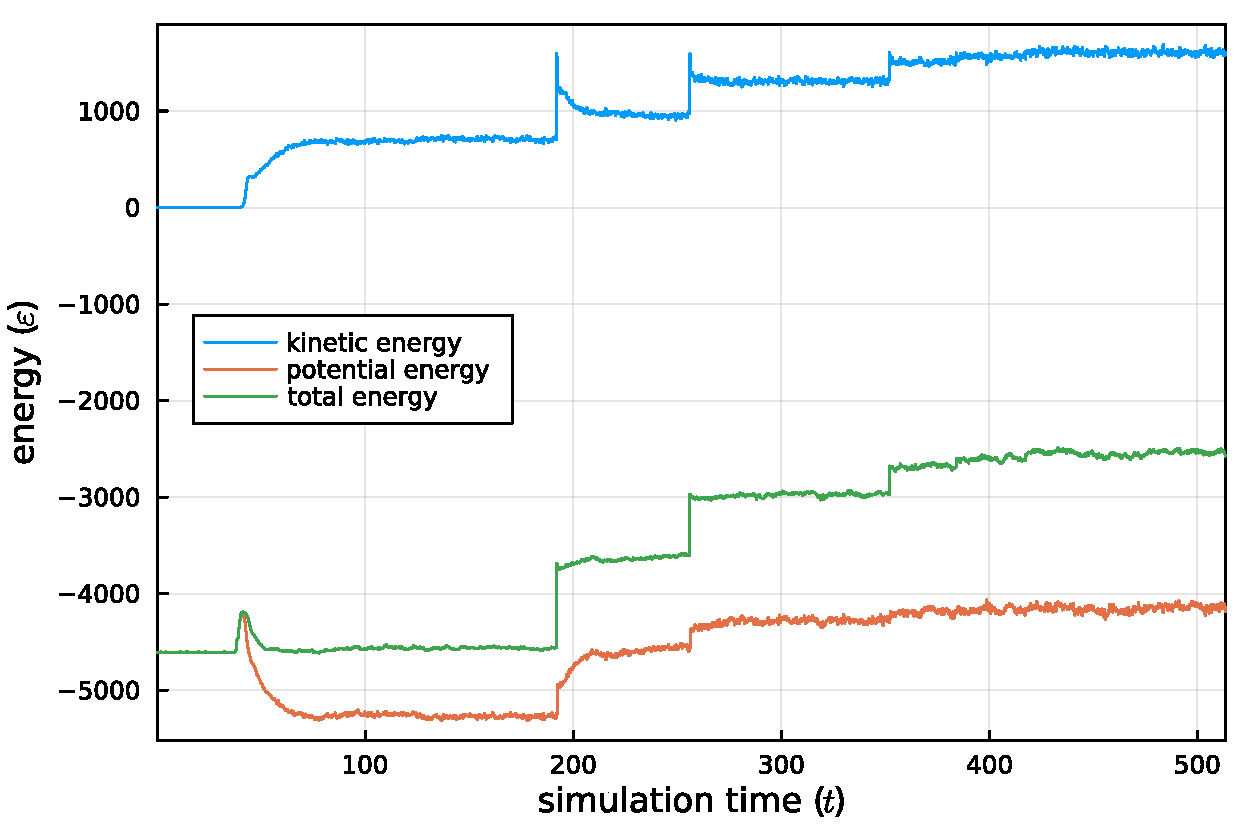
\includegraphics[width=0.8\textwidth]{e-t-thermostat}
    \caption{The dimensionless kinetic energy, potential energy, and total energy
        as a function of simulation time $t$ after applying the velocity-rescaling
        thermostat for several times.}
    \label{fig:md-thermostat}
\end{figure}

We also plot Figure~\ref{fig:T-t} to show the change of temperatures as a function
of the simulation time.

\begin{figure}
    \centering
    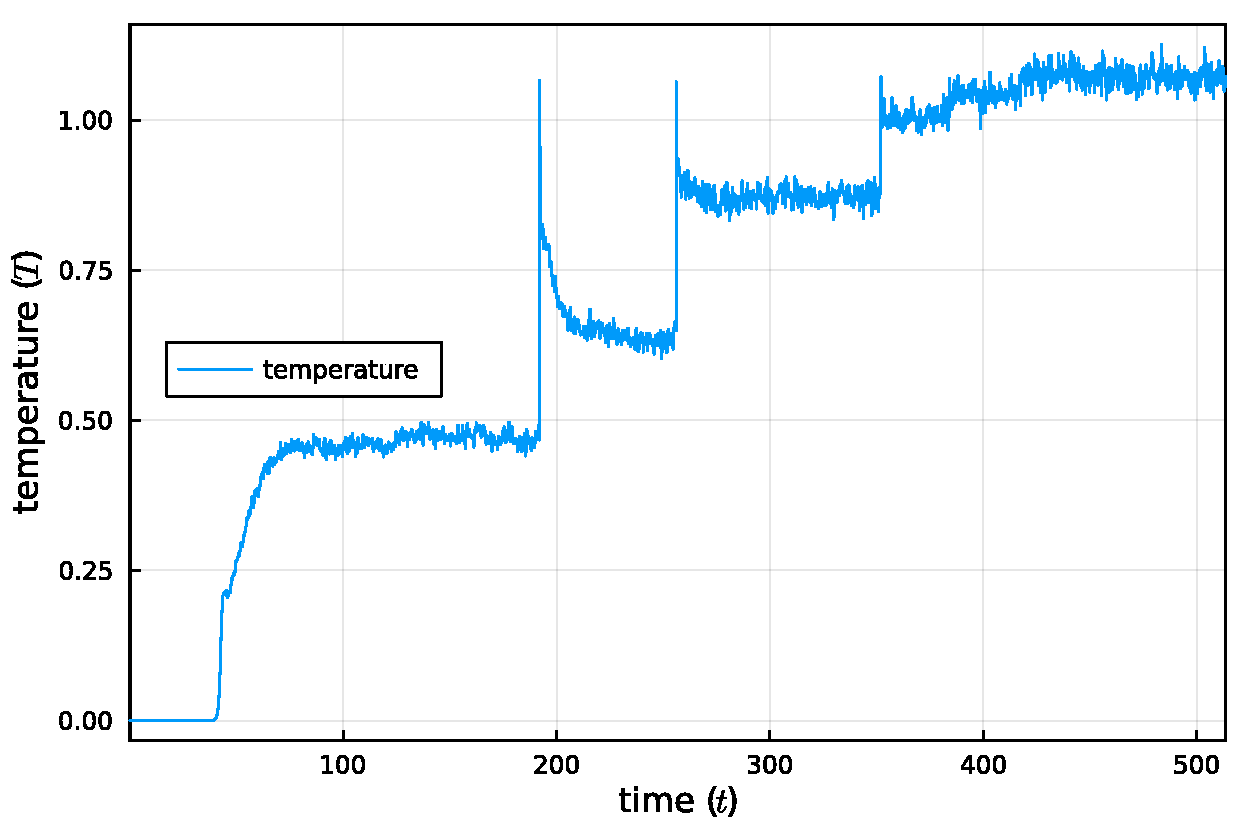
\includegraphics[width=0.8\textwidth]{T-t}
    \caption{The dimensionless temperature as a function of simulation time $t$ after
        applying the velocity-rescaling thermostat for several times.}
    \label{fig:T-t}
\end{figure}

\subsection{Calculation results}

\begin{figure}[H]
    \centering
    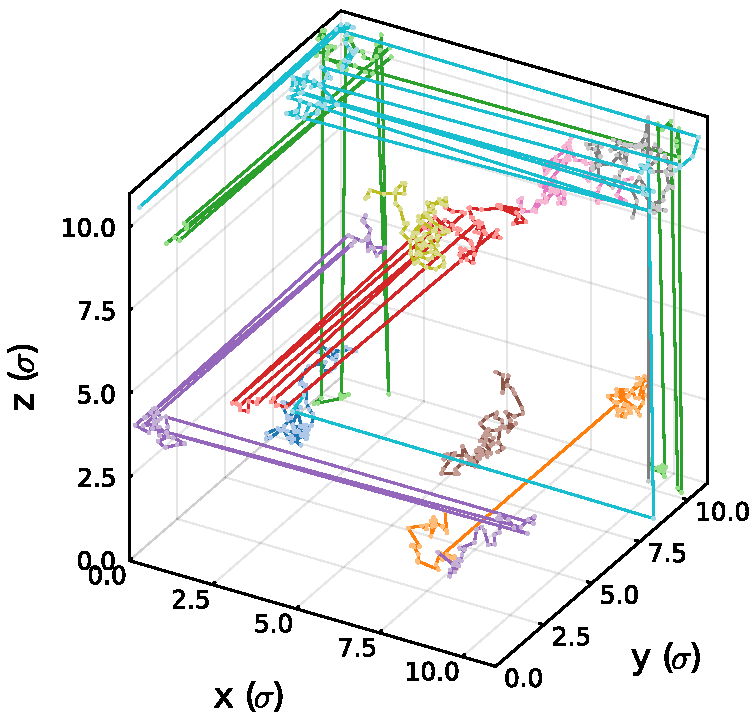
\includegraphics[width=0.8\textwidth]{traces}
    \caption{The traces of the \(100\)th to \(1000\)th particles from \(t = 390\) to \(t = 500\).}
    \label{fig:traces}
\end{figure}

We select several particles (\(100\)th, \(200\)th, \(\ldots\), \(1000\)th) and plot their traces
from \(t = 390\) to \(t = 500\) (i.e., at \(T \approx 1.073\)) in Figure~\ref{fig:traces}.
The figure shows that these particles are wandering around a certain
range. The straight lines passing through the box does not mean they just at a very
large speed, since after thermalization, the speed of particles would not change so
much. These lines just indicate that these particles move out the current cell,
and their images reappear from the other side of the cell, as required by the PBCs.

Now let us calculate the \ce{Ar} system's thermodynamic properties.
The pressure is calculated from the virial theorem, as shown in~\eqref{eq:P}
%
\begin{equation}\label{eq:P}
    \frac{ P }{ \rho k_B T } = 1 - \frac{ 1 }{ 3N k_B T } \sum_{i=1}^{N}
    \sum_{\alpha=1}^{3}
    \biggl \langle r_i^\alpha \frac{ \partial u }{ \partial r_i^\alpha } \biggr \rangle,
\end{equation}
%
where \(\langle \cdot \rangle\) denotes the time or ensemble average,
and \(i\) labels all the particles, and \(\alpha\) labels the three spatial dimensions.
Since the virial part is derived from \(u\), so the second term we get from our code
is already in unit of \(k_B\). Theferfore, the actual code is
equivalent to
%
\begin{equation}\label{eq:P}
    \frac{ \beta P }{ \rho } = 1 + \frac{ 1 }{ 3N T } \sum_{i=1}^{N}
    \langle \bm{r}_i \cdot \bm{F}_i \rangle,
\end{equation}
%
where \(\beta = \nicefrac{ 1 }{ k_B T }\) in Verlet's paper\cite{Verlet},
which is \(0.90\) at \(\rho = 0.75\) and \(T = 1.069\).

We pick steps from \(15000\) to the last step (total \(1046\) steps) and do the time average,
what we get is \(\nicefrac{ \beta P }{ \rho } \approx 0.80402\), which is quite
different from \(0.90\).

The Maxwell velocity distribution is
%
\begin{equation}
    f(v) = \biggl( \frac{m}{2\pi k_B T} \biggr)^{3/2}
    4\pi v^2 \exp{\biggl( -\frac{m v^2}{2 k_B T} \biggr)},
\end{equation}
%
where \(f(v)\) is a probability distribution function, and \(v\) is the magnitude of the
velocity vector.
We plot histograms of velocity distribution of the particles after
\(500\), \(1000\), \(2000\), \(3000\), \(5000\), \(8000\), \(10000\), \(12000\), \(16000\) steps,
respectively, in Figure~\ref{fig:maxwell}.
%
\begin{figure}
    \centering
    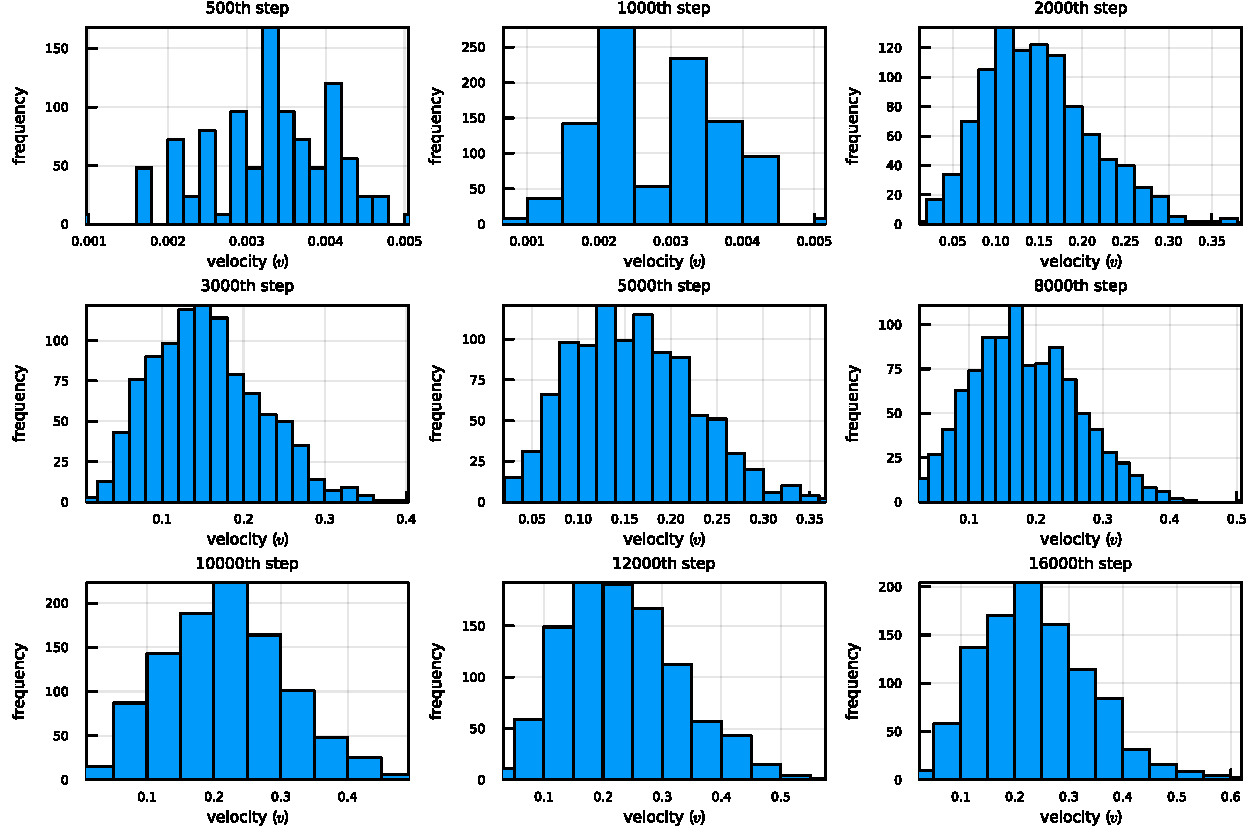
\includegraphics[width=\textwidth]{maxwell}
    \caption{Histograms of velocity distribution of the particles after
        \(500\), \(1000\), \(2000\), \(3000\), \(5000\), \(8000\), \(10000\), \(12000\), \(16000\) steps.}
    \label{fig:maxwell}
\end{figure}
%
We can see that at the beginning of the computation, the velocities of the particles
seem to be random, but as the number of time steps increases, a pattern starts to
emerge. After the \(5000\)th step (\(t = 160\)), we can almost see a Maxwell distribution.
From the \(10000\)th (\(t = 320\)) to the \(16000\)th (\(t = 512\)) steps, the pattern is
already Maxwellian and does not change so much.


\clearpage
\bibliographystyle{elsarticle-num}
\bibliography{ref}

\end{document}
